\documentclass[11pt,a4paper]{article}
\usepackage[margin=2.1cm,top=2.5cm,headheight=26pt]{geometry}
\usepackage{amsmath,amssymb,bm}
\usepackage{siunitx}
\usepackage{booktabs}
\usepackage{graphicx}
\usepackage{tikz}
\usetikzlibrary{arrows.meta,calc,positioning}
\usepackage{enumitem}
\usepackage{float}
\usepackage{xcolor}
\usepackage{fancyhdr}
\usepackage{tcolorbox}
\tcbuselibrary{skins,breakable}
\usepackage[colorlinks=true,linkcolor=blue!60!black,urlcolor=blue!60!black]{hyperref}
\sisetup{per-mode=symbol,detect-all}
\graphicspath{{figs/}}

% Photograph slot: renders the image if the file is present in figs/,
% otherwise a dashed placeholder box telling you which file to drop in.
% #1 = file name (no extension), #2 = width fraction, #3 = caption, #4 = what the picture should be
\newcommand{\photo}[4]{%
  \begin{figure}[H]\centering
  \IfFileExists{figs/#1.jpg}{\includegraphics[width=#2\linewidth]{#1}}{%
  \IfFileExists{figs/#1.png}{\includegraphics[width=#2\linewidth]{#1}}{%
    \begin{tikzpicture}
      \draw[dashed,gray,line width=0.8pt] (0,0) rectangle (#2\linewidth,0.52*#2\linewidth);
      \node[align=center,text width=0.82*#2\linewidth,font=\footnotesize\itshape,gray!70!black]
        at (0.5*#2\linewidth,0.26*#2\linewidth) {PHOTOGRAPH: #4\\[3pt]\ttfamily figs/#1.jpg};
    \end{tikzpicture}}}
  \caption{#3}
  \end{figure}}

\definecolor{navy}{RGB}{25,53,73}
\newtcolorbox{keybox}[1]{title={#1},colback=blue!4,colframe=blue!50!black,fonttitle=\bfseries,breakable}
\newtcolorbox{aerobox}[1]{title={#1},colback=orange!5,colframe=orange!60!black,fonttitle=\bfseries,breakable}
\newtcolorbox{sumbox}[1]{title={#1},colback=green!4,colframe=green!40!black,fonttitle=\bfseries,breakable}

\pagestyle{fancy}
\fancyhf{}
\lhead{
\includegraphics[height=0.6cm]{logos/itu_logo_laci.pdf}\ \ UCK 364E Design of Machine Elements}
\rhead{Case Study 1 --- Handout}
\lfoot{\footnotesize Department of Aeronautical Engineering, Istanbul Technical University}
\rfoot{\footnotesize Page \thepage}

\begin{document}

\begin{center}
{\Large\textbf{Case Study: BOAC Flight 781 and the de Havilland Comet}}\\[3pt]
{\large\textbf{How fatigue at a stress concentration destroyed the world's first jet airliner}}\\[5pt]
{\small Prof.\ Dr.\ Onur Tunçer \ $\cdot$\ UCK 364E Design of Machine Elements}
\end{center}

\vspace{2pt}\hrule\vspace{6pt}

\noindent\emph{Why you are reading this.} Every concept in the first weeks of this course --- limit and ultimate load, factor of safety, stress concentration, fatigue, damage tolerance, full-scale testing --- exists in its present form largely because of this accident. It is the clearest example you will meet of a structure that passed every static strength check and still broke apart.

\section{What happened}

On \textbf{10 January 1954}, a de Havilland Comet 1 registered \textbf{G-ALYP}, operating BOAC Flight 781 from Singapore to London, took off from Rome--Ciampino on the last leg of the route. Roughly twenty minutes later the aircraft suffered an explosive decompression at altitude, broke up in mid-air and fell into the Mediterranean near the island of Elba. All 35 people on board --- 29 passengers, including ten children, and 6 crew --- were killed.

\photo{g-alyp}{0.50}{De Havilland Comet 1 G-ALYP, the aircraft lost on 10 January 1954. It was the third Comet built and the first to carry fare-paying jet passengers, in May 1952.}{G-ALYP in BOAC livery before the accident}

It was not an isolated event. It was the second of three fatal Comet accidents in under twelve months, all caused by structural failure: BOAC Flight 783 near Calcutta in May 1953, Flight 781 in January 1954, and \textbf{South African Airways Flight 201} (G-ALYY) on 8 April 1954, lost after departing from the same Rome airport in closely similar circumstances. The Comet fleet had been returned to service on 23 March 1954, only ten weeks after the first loss and before the cause was understood; the second accident followed sixteen days later.

\section{How the cause was found}

This was the investigation that effectively invented modern accident investigation. In 1954 there were no flight data recorders, no cockpit voice recorders and no established investigation protocol, and the wreckage lay on the sea floor. The pieces of the method are worth knowing:

\begin{description}[nosep,leftmargin=0.6cm,style=nextline]
  \item[Recovery.] Royal Navy vessels and a civilian salvage ship recovered the wreckage, using underwater television cameras developed for the purpose --- a first.
  \item[Pathology.] The post-mortem findings were fractured skulls and ruptured lungs, with no evidence of an explosion or fire. Ruptured lungs point unambiguously to rapid decompression; a reconstruction with a model fuselage and dummies showed that occupants were thrown head-first into the cabin ceiling at the instant of rupture.
  \item[Reconstruction.] The recovered structure was laid out at the Royal Aircraft Establishment at Farnborough. Carpet fibres trapped in the tail, the imprint of a coin on a rear fuselage panel, and seat paint smeared along the rear fuselage all showed that the cabin had burst and its contents had been blown aft \emph{in flight}.
  \item[The water-tank test.] BOAC gave up a sister aircraft, G-ALYU, which was immersed in a water tank and pressurised and depressurised repeatedly, around the clock, to simulate flight cycles. After the equivalent of about 3\,000 flights the fuselage failed in the tank.
\end{description}

\photo{rae-reconstruction}{0.52}{Which parts of G-ALYP were recovered (shaded), and the location of the forward ADF aerial aperture in the cabin roof where the failure began. Laying out every recovered fragment in its original position showed the order in which the structure came apart and pointed back to the first failure.}{plan view of the recovered wreckage with the ADF aperture marked}

\begin{keybox}{Why a \emph{water} tank?}
Pressurising a cabin with air stores an enormous amount of energy ($\sim pV$ of a compressible fluid); when it bursts, the structure is destroyed and the evidence with it. Water is practically incompressible, so the stored energy is tiny: the structure simply splits and can then be examined, measured and fractographically analysed. Full-scale fatigue test articles have been tested this way ever since.
\end{keybox}

\photo{water-tank}{0.50}{G-ALYU in the water tank at Farnborough. The whole fuselage was submerged and the cabin pressurised and depressurised around the clock; it failed after the equivalent of about 3\,000 flights, from a corner of a cabin-roof aperture --- exactly as G-ALYP had.}{the full-scale water-tank fatigue test of G-ALYU}

\section{The engineering cause}

The Court of Inquiry reported jointly on both accidents on 1 February 1955. The cabin had failed by \textbf{metal fatigue}, starting at the corner of a window aperture in the cabin roof --- an opening for the ADF (radio navigation) aerial, closed with a fibreglass panel rather than glass. Three things combined:

\begin{enumerate}[nosep]
  \item \textbf{Cyclic loading.} Each flight is one full pressurisation cycle: the cabin is inflated on climb and deflated on descent. The hoop stress $\sigma_\theta=pr/t$ therefore swings from zero to its maximum once per flight, plus the flight loads superimposed on it. Fatigue damage accumulates flight by flight.
  \item \textbf{Stress concentration.} The window aperture was a cut-out in a pressurised shell. The local stress at its corner is $K_t$ times the nominal hoop stress, and $K_t$ rises sharply as the corner radius falls.
  \item \textbf{Manufacturing defects.} The aperture surrounds were \emph{riveted} where the original design had called for them to be bonded, and the holes were made by \textbf{punch riveting} rather than drilling. Punching leaves a torn, imperfect hole with small cracks already present at its edge --- so the crack-initiation phase was effectively skipped and cracks began to grow from the first flights.
\end{enumerate}

\photo{fatigue-origin}{0.52}{The surviving cabin-roof section of G-ALYP, on display at the Science Museum, London. The two rectangular apertures are the ADF aerial windows; the fatigue crack that destroyed the aircraft grew from the rivet holes at the corner of one of them.}{the preserved G-ALYP cabin-roof section with the ADF apertures}

\begin{aerobox}{The point that matters most for this course}
The Comet's pressure cabin was \emph{not} weak. The British airworthiness requirement of the day was a proof pressure of $1.33P$ and an ultimate of $2P$; de Havilland designed the Comet cabin to $2.5P$ --- comfortably stronger than required, and it had been pressure-tested successfully. The aircraft had an excellent \emph{static} margin of safety and still failed after a few thousand flights.

\medskip
\textbf{A positive static margin of safety says nothing about fatigue life.} They are separate checks, and for a pressurised fuselage the fatigue check is the one that sizes the structure.
\end{aerobox}

\section{The physics, in the symbols you already use}

For a thin-walled cylinder, the hoop and longitudinal stresses from the cabin differential pressure $\Delta p$ are
\[
\sigma_\theta=\frac{\Delta p\,r}{t},\qquad \sigma_z=\frac{\Delta p\,r}{2t}.
\]
The local stress at the corner of a cut-out is $\sigma_{\max}=K_t\,\sigma_{\text{nom}}$, where for a circular hole in a wide plate under uniaxial tension $K_t=3$; for a square corner $K_t$ is far higher and tends to infinity as the corner radius $r_c\to 0$. In fatigue the relevant quantity is the notch factor $K_f=1+q(K_t-1)$, which for a thin, ductile skin is close to $K_t$ itself. The alternating stress that drives crack growth is therefore of order $K_f\,\sigma_\theta/2$ --- several times the nominal stress the designer checked.

\begin{figure}[H]\centering
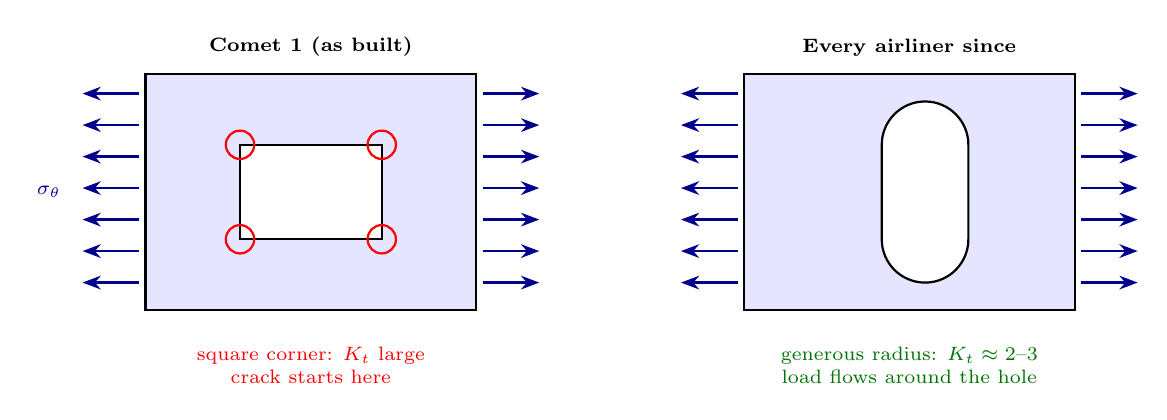
\begin{tikzpicture}[scale=1.0,>=Stealth,font=\scriptsize]
% --- square window
\begin{scope}
\fill[blue!10] (0,0) rectangle (4.2,3.0);
\draw[thick] (0,0) rectangle (4.2,3.0);
\fill[white] (1.2,0.9) rectangle (3.0,2.1);
\draw[thick] (1.2,0.9) rectangle (3.0,2.1);
\foreach \y in {0.35,0.75,...,2.8} {\draw[->,thick,blue!55!black] (-0.08,\y) -- (-0.8,\y);}
\foreach \y in {0.35,0.75,...,2.8} {\draw[->,thick,blue!55!black] (4.28,\y) -- (5.0,\y);}
\draw[red,thick] (1.2,2.1) circle (0.18); \draw[red,thick] (3.0,2.1) circle (0.18);
\draw[red,thick] (1.2,0.9) circle (0.18); \draw[red,thick] (3.0,0.9) circle (0.18);
\node[red,align=center,anchor=north] at (2.1,-0.35) {square corner: $K_t$ large\\ crack starts here};
\node[anchor=south] at (2.1,3.1) {\textbf{Comet 1 (as built)}};
\node[blue!55!black,anchor=east] at (-0.95,1.5) {$\sigma_\theta$};
\end{scope}
% --- rounded window
\begin{scope}[xshift=7.6cm]
\fill[blue!10] (0,0) rectangle (4.2,3.0);
\draw[thick] (0,0) rectangle (4.2,3.0);
\fill[white] (1.75,0.9) arc (180:360:0.55 and 0.55) -- (2.85,2.1) arc (0:180:0.55 and 0.55) -- cycle;
\draw[thick] (1.75,0.9) arc (180:360:0.55 and 0.55) -- (2.85,2.1) arc (0:180:0.55 and 0.55) -- cycle;
\foreach \y in {0.35,0.75,...,2.8} {\draw[->,thick,blue!55!black] (-0.08,\y) -- (-0.8,\y);}
\foreach \y in {0.35,0.75,...,2.8} {\draw[->,thick,blue!55!black] (4.28,\y) -- (5.0,\y);}
\node[green!45!black,align=center,anchor=north] at (2.1,-0.35) {generous radius: $K_t\approx 2$--3\\ load flows around the hole};
\node[anchor=south] at (2.1,3.1) {\textbf{Every airliner since}};
\end{scope}
\end{tikzpicture}
\caption{Why airliner windows are round. The aperture is a cut-out in a shell carrying hoop stress; the sharper the corner, the higher the local stress and the shorter the fatigue life.}
\end{figure}

\section{What changed because of it}

\begin{itemize}[nosep]
  \item \textbf{Rounded apertures.} Windows, doors and hatches in pressurised structure are given generous corner radii. The Comet 1 never flew again, but later Comet marks, with rounded windows, served for thirty years.
  \item \textbf{Fatigue became a certification requirement.} Pressure-cabin strength requirements were revised, and the demonstration of fatigue life --- not merely static strength --- entered the airworthiness codes. The modern descendant is \textbf{CS-25.571 / FAR 25.571}, ``Damage tolerance and fatigue evaluation of structure''.
  \item \textbf{The full-scale fatigue test.} Testing a complete airframe in a water tank for the equivalent of several design lives became standard practice, and remains so.
  \item \textbf{Hole quality is a design parameter.} Punch riveting was abandoned for fatigue-critical structure in favour of drilled and reamed holes, and later cold-expanded holes and interference-fit fasteners.
  \item \textbf{Damage tolerance.} The deeper shift came later: rather than assuming a structure is crack-free, assume cracks exist and schedule inspections so they are found before they become critical.
\end{itemize}

\begin{sumbox}{Five lines to remember}
\begin{enumerate}[nosep]
  \item A large static margin of safety does not protect against fatigue.
  \item One flight $=$ one pressurisation cycle; a fuselage accumulates tens of thousands of them.
  \item Fatigue cracks start at the surface, at a stress concentration, almost always at a hole or a corner.
  \item How a hole is \emph{made} matters as much as where it is placed.
  \item If you cannot prove the life by analysis, you test it --- full scale, to several design lives.
\end{enumerate}
\end{sumbox}

\section{Questions to think about}

\begin{enumerate}[nosep]
  \item A cabin of radius \SI{1.5}{m} and skin thickness \SI{0.9}{mm} operates at $\Delta p=\SI{57}{kPa}$. Compute the hoop stress, then the ultimate margin of safety against $F_{tu}=\SI{434}{MPa}$ for 2024-T3. Does the number surprise you, given that the aircraft broke apart?
  \item The same cabin has a window corner with $K_t=5$ instead of $K_t=2.5$. By roughly what factor does the local alternating stress change, and --- using a typical S--N slope of $S_a\propto N^{-0.13}$ --- by what factor does the life change?
  \item The Comet fleet returned to service ten weeks after the first accident, before the cause was known. What should have been required before that decision, and which of the three philosophies in CS-25.571 does the decision violate?
  \item Punched holes contain pre-existing cracks. Which of the three stages of fatigue does this eliminate, and why does that matter so much for total life?
\end{enumerate}

\section*{Sources and image credits}
\footnotesize
\textbf{Photographs.} Images reproduced from Wikimedia Commons / the Wikipedia article on BOAC Flight 781 and the Court of Inquiry report. The individual licence of each image should be verified before the handout is distributed beyond the class, and the credit line completed here. Source files live in the \texttt{figs/} folder beside this \texttt{.tex}; replace any of them with a higher-resolution copy of the same subject and the document recompiles unchanged.

\medskip
\emph{Civil Aircraft Accident: Report of the Court of Inquiry into the Accidents to Comet G-ALYP on 10 January 1954 and Comet G-ALYY on 8 April 1954}, HMSO, 1 February 1955 --- \href{https://www.faa.gov/sites/faa.gov/files/2022-10/G-ALYP_Report_0.pdf}{the original report (FAA archive)}. \ FAA, \emph{Lessons Learned from Transport Airplane Accidents}. \ Wikipedia, \href{https://en.wikipedia.org/wiki/BOAC_Flight_781}{BOAC Flight 781} (summary and figures above drawn from it).

\end{document}
